\let\negmedspace\undefined
\let\negthickspace\undefined
\documentclass[journal]{article}
\usepackage[a5paper, margin=10mm, onecolumn]{geometry}
\usepackage{lmodern} % Ensure lmodern is loaded for pdflatex

\setlength{\headheight}{1cm} % Set the height of the header box
\setlength{\headsep}{0mm}     % Set the distance between the header box and the top of the text

\usepackage{gvv-book}
\usepackage{gvv}
\usepackage{cite}
\usepackage{textcomp}
\usepackage{amsmath,amssymb,amsfonts,amsthm}
\usepackage{algorithmic}
\usepackage{graphicx}
\graphicspath{{./figs/}}
\usepackage{textcomp}
\usepackage{xcolor}
\usepackage{txfonts}
\usepackage{listings}
\usepackage{enumitem}
\usepackage{mathtools}
\usepackage{gensymb}
\usepackage{comment}
\usepackage[breaklinks=true]{hyperref}
\usepackage{tkz-euclide} 
\usepackage{listings}
\usepackage{gvv}                                        
\def\inputGnumericTable{}                                 
\usepackage[latin1]{inputenc}                                
\usepackage{color}                                            
\usepackage{array}                                            
\usepackage{longtable}                                       
\usepackage{calc}                                             
\usepackage{multirow}                                         
\usepackage{hhline}                                           
\usepackage{ifthen}                                           
\usepackage{lscape}
\usepackage{circuitikz}
\tikzstyle{block} = [rectangle, draw, fill=blue!20, 
text width=4em, text centered, rounded corners, minimum height=3em]
\tikzstyle{sum} = [draw, fill=blue!10, circle, minimum size=1cm, node distance=1.5cm]
\tikzstyle{input} = [coordinate]
\tikzstyle{output} = [coordinate]


\begin{document}
	
	\bibliographystyle{IEEEtran}
	\vspace{3cm}
	
\title{4.13.51}
\author{EE25BTECH11047 - RAVULA SHASHANK REDDY}
\maketitle
\hrulefill
\bigskip 

\renewcommand{\thetable}{\theenumi}
\setlength{\intextsep}{10pt}

\textbf{Question:} \\

One of the diameters of the circle circumscribing the rectangle \(ABCD\) is given by
\begin{align*}
4y = x + 7.
\end{align*}

If \(\vec{A}=(-3,4)\) and \(\vec{B}=(5,4)\), find the area of the rectangle.\\

\textbf{Solution:}

\begin{align}
\vec{A}=\myvec{-3\\4},\quad \vec{B}=\myvec{5\\4}
\end{align}

Centre \(\vec{O}\) lies on the diameter and also on the perpendicular bisector of chord passing  

through \(\vec{A}\) and \(\vec{B}\).\\

Perpendicular Bisector equation:
\begin{align}
\myvec{1 \\ 0}^T\vec{x}&=1
\end{align}

Diameter equation:
\begin{align}
\myvec{1 \\ -4}^T\vec{x}&=-7\\
\therefore
\myvec{1 & 0\\ 1 & -4}\vec{O} &= \myvec{1\\-7}
\end{align}
\begin{align}
\myvec{1 & 0 & 1\\[4pt] 1 & -4 & -7}
\xrightarrow{R_2\rightarrow R_2-R_1}
\myvec{1 & 0 & 1\\[4pt] 0 & -4 & -8}
\xrightarrow{R_2\rightarrow (-\tfrac{1}{4})R_2}
\myvec{1 & 0 & 1\\[4pt] 0 & 1 & 2}
\end{align}
\begin{align}
    \vec{O}=\myvec{1\\2}
\end{align}

Radius of circumcircle
\begin{align}
r&=||\vec{O}-\vec{A}||=2\sqrt{5}
\end{align}

Hence the Circumcircle equation is:
\begin{align}
||\vec{x}||^2+2\vec{c}^T\vec{x}+f&=0\\
\vec{c}&=-\vec{O}\\
f&=||\vec{c}||^2-r^2=-15
\end{align}
\begin{center}
\begin{align}
\boxed{||\vec{x}||^2+2\myvec{-1 & -2}\vec{x}-15=0}
\end{align}
\end{center}
\begin{align}
\vec{C}&=2\vec{O}-\vec{A}=\myvec{2\\4}-\myvec{-3\\4}=\myvec{5\\0},\\
\vec{D}&=2\vec{O}-\vec{B}=\myvec{2\\4}-\myvec{5\\4}=\myvec{-3\\0}.
\end{align}
\begin{align}
\vec{B}-\vec{A}=\myvec{8\\0},\qquad
\vec{D}-\vec{A}=\myvec{0\\-4}.
\end{align}

\begin{align}
\text{Area} &= \big|\vec{B}-\vec{A}\times\vec{D}-\vec{A}\big|
= \left|\det\myvec{8 & 0\\[4pt]0 & -4}\right|
= |8(-4)-0| = 32.
\end{align}
\newpage
\begin{figure}
    \centering
    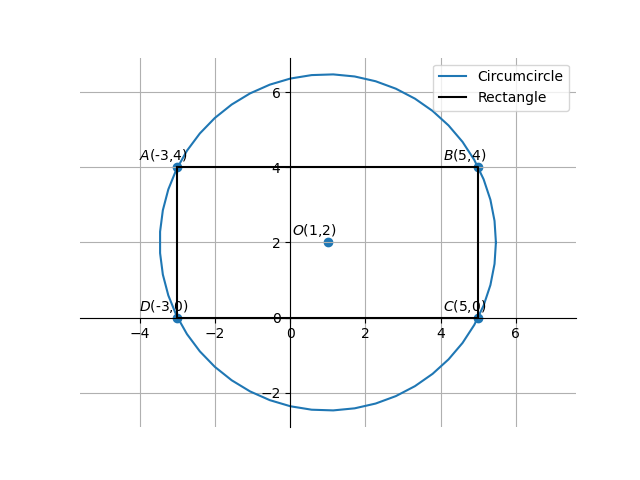
\includegraphics[width=1.0\linewidth]{figs/fig1.png}
    \caption{}
    \label{fig:placeholder}
\end{figure}
\end{document}